\documentclass[12pt]{article}
\usepackage{pagestyle}

\begin{document}
\thispagestyle{empty}

{\scshape ML } \hfill {\scshape \large Lecture 4 - Probalistic models} \hfill {\scshape 20.02.2024}
 
\smallskip
\hrule
\bigskip

%table of contents 
\tableofcontents

\section{Learning}

\subsection{The machine analogy}

We assume a machine which has a configuration specified by a set of parameters $\Theta$ that produces some output Data $D$. We understand how the machine works so the probability of some $D$ given $\theta$ is known. But since we observe the data we want to know the probability of some configuration $\theta$ given the data $D$. The machine here in practice is often a probability distribution.

\subsection{Frequentist learning}

\begin{definition}[Frequentist learning]
    In frequentist learning we are given some data and our job is to guess the true model (out of a set of models) that generated some data. In other words, we want to pick the right $\theta$ so that the probability distribution fits the data best.
\end{definition}

\begin{definition}[Maximum likelihood]
    The maximum likelihood estimate/principle is the model criteria for which we guess the model for which the probability of seeing the data that we saw is the highest. Formally, this is given by 
    \[
        \hat{\theta} = \arg\max_{\theta} P(D|\theta)  
    \]
    this just expresses that our configuration $\hat{\theta}$ is the one that maximizes the probability of seeing the data $D$ given $\theta$.
\end{definition}

\subsubsection*{Coinflip example - model selection problem}

There is a straight and a bent coin. Without telling us a friend picks up one of the coins and flips it 12 times. This yields the following probabilities.

\begin{figure}[!h]
    \centering
    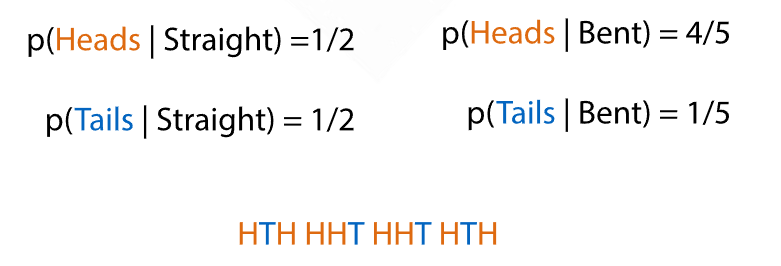
\includegraphics[width=0.5\textwidth]{assets/coinflip.png}
\end{figure}

Some notes regarding this example: 
\begin{itemize}[leftmargin=*, noitemsep]
    \item the model class conists of the two coins: straight and bent
    \item the data consits of 12 instances: the 12 coin flips
    \item the coins are a Bernoulli distribution with the parameters $\frac{1}{2}$ and $\frac{4}{5}$
\end{itemize}

The maximum liklihood estimation here can be expressed as: 
\begin{align*}
    \argmax_{\text{Coin}\in\{\text{Bent}, \text{Straight}\}} & p(HTHHHTHHTHTH\mid \text{Coin}) \\
    \argmax_{\text{Model}\in \text{Model space}} & p(D\mid \text{Model})
\end{align*}
Here we just compute $p(D\mid \text{Bent})$ and $p(D\mid \text{Straight})$ and pick the one that is higher. We have that 

\begin{align*}
    p(D\mid \text{Bent}) & \approx 0.000286 \\ 
    p(D\mid \text{Straight}) & \approx 0.000244
\end{align*}

From which we can conclude that we would prefer the bent coin model for the observed data.

\subsubsection*{Estimating mean example}

Another example would be wanting to find the maximum likelihood estimate for the mean of a normal distribution given some data.

\begin{figure}[!h]
    \centering
    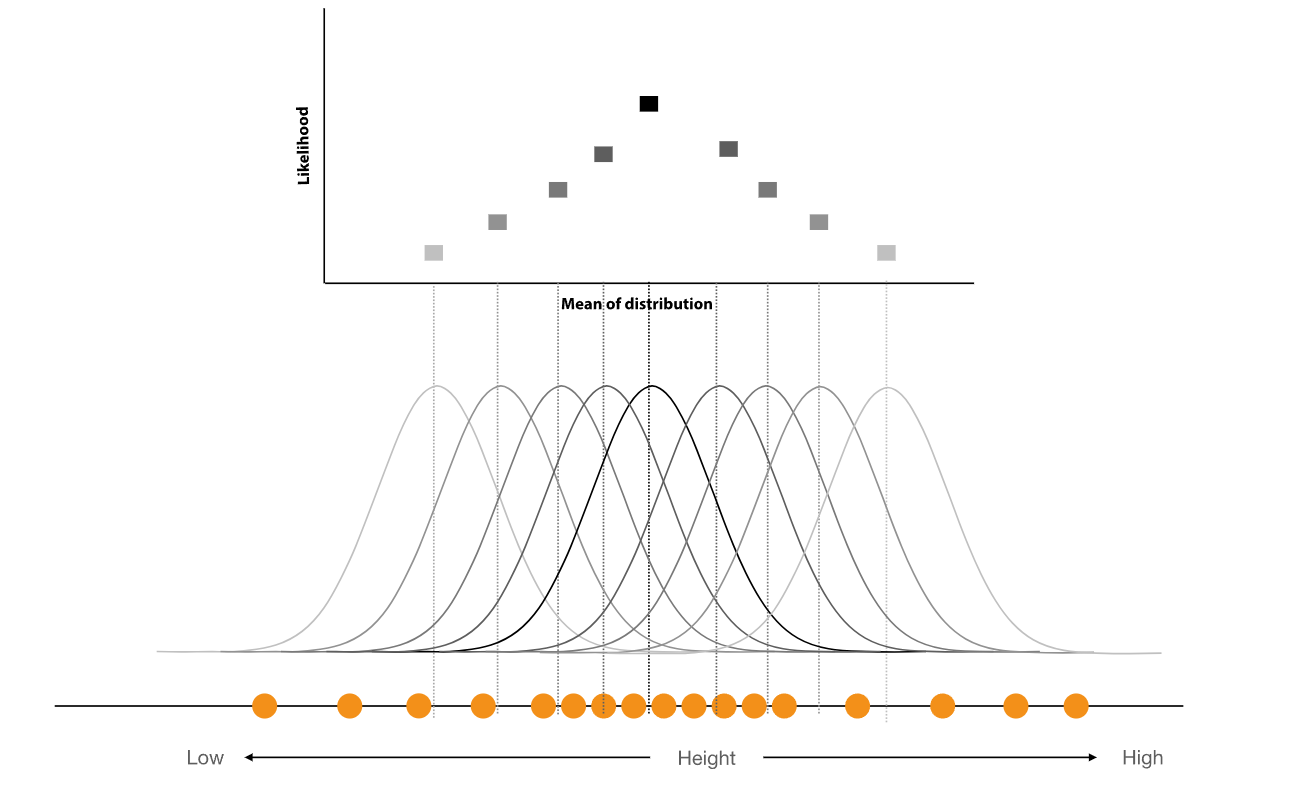
\includegraphics[width=0.6\textwidth]{assets/maximumlikeli.png}
\end{figure}

\subsection{Log-likelihood (loss)}

\begin{definition}[log-likelihood]
    The log-likelihood is the logarithm of the maximum likelihood function. It shares the maxima and is easier to symbolically maniuplate. It also provides a smoother loss surface for methods like gradient descent. Usually we take the \textit{negative} log-likelihood, so that we can preform gradient descent to find the optimum.
\end{definition}


\subsection{Maxmium likelihood for normal distribution}

Formally we can express the maximum likelihood estimate for the mean of a normal distribution as follows.
\begin{align*}
    \argmax_{\theta} \ln p(X\mid \theta) & = \argmax_{\theta} \ln \prod_{x\in X} p(x\mid \theta) \\
    & = \argmax_{\theta} \sum_{x\in X} \ln p(x\mid \theta) \quad p(x\mid \theta) = N(x\mid \mu, \sigma) \\
    & = \argmax_{\mu, \sigma} \sum_{x} \ln\left[  \frac{1}{\sqrt{2\pi\sigma^2}} \exp\left(-\frac{(x-\mu)^2}{2\sigma^2}\right) \right]\\
    & = \argmax_{\mu, \sigma} \sum_{x} \ln \left[ \frac{1}{\sqrt{2\pi\sigma^2}} -\frac{(x-\mu)^2}{2\sigma^2}\right]\\
\end{align*}

We can graph the landscape of the log-likelihood function as follows. 
\begin{figure}[!h]
    \centering
    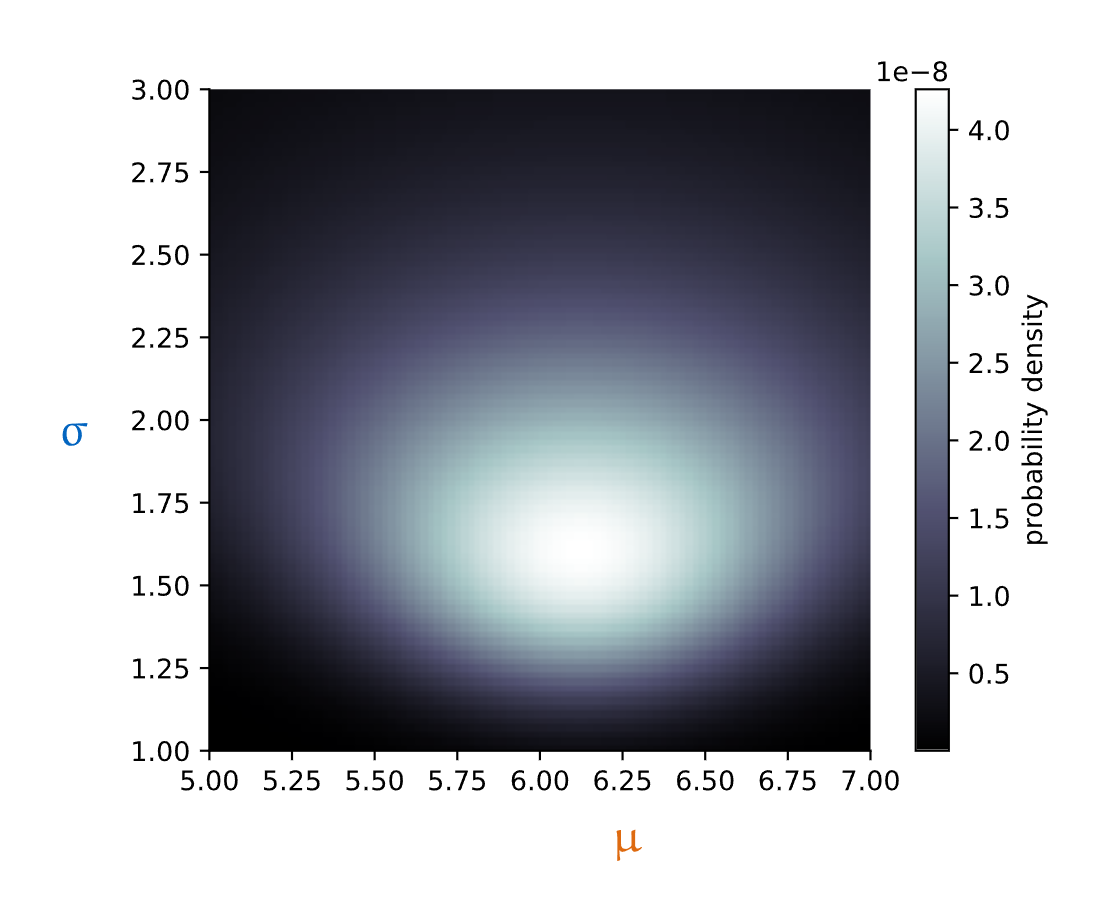
\includegraphics[width=0.5\textwidth]{assets/probdensity.png}
\end{figure}

Some notes regarding this landscape: 
\begin{itemize}[leftmargin=*, noitemsep]
    \item The mean and variance that give us a model which best fits our data are in the bright spot.
    \item If we don't want to do an analytic solution we could find the optimum by using gradient descent or random search.
\end{itemize}

\subsubsection*{Removing parameters}

If we remove each parameter we can further simplify the problem, for example the maximum likelihood estimate for just the mean is given by 
\begin{align*}
    \argmax_{\mu} \sum_{x} \ln N(x\mid \mu, \sigma) & = \argmax_{\mu} \sum_{x} -\frac{(x-\mu)^2}{2\sigma^2} \quad \text{(constant rule)}\\
    & = \argmax_{\mu} -\frac{1}{2\sigma^2} \sum_{x} (x-\mu)^2 \quad \text{(constant rule)}\\
    & = \argmax_{\mu} - \sum_{x} (x-\mu)^2 \quad \text{(constant rule)}\\ 
    & = \argmin_{\mu} \sum_{x} (x-\mu)^2
\end{align*}

The maximum likelihood estimate for the mean is just the value that minimizes the sum of the squared differences between the data and the mean. The key insight here being that even if a likelihood function looks complex its often the case when you take the logarithm and maximize it the complexity dissapears.

\subsection{Bayesian learning}

We can break the bayesian learning formula into the following components: 
\[
    \underbrace{p(\theta\mid D)}_{\text{posterior d.}} = \underbrace{p(D)^{-1}}_{\text{model evidence}} \underbrace{p(D\mid \theta)}_{\text{data d.}} \underbrace{p(\theta)}_{\text{prior d.}}
\]

Where 
\begin{itemize}[leftmargin=*, noitemsep]
    \item posterior distribution: a distribution over all possible models given some data we observed $D$
    \item prior distribution: our belief about the model before we see the data 
\end{itemize}

\subsubsection*{Coinflip example}

Using the coinflip example again the first thing we want to calculate is the prior distribution. We can express this as: 
\begin{align*}
    p(D) & = p(D, \text{Bent}) + p(D, \text{Straight}) \\
    & = p(D\mid \text{Bent})p(\text{Bent}) + p(D\mid \text{Straight})p(\text{Straight}) \\
\end{align*}

We can then sub the above result into the bayesian learning formula to get the posterior distribution for the Straight model as:
\begin{align*}
    p(\text{Straight}\mid D) & = \frac{p(D\mid \text{Straight})p(\text{Straight})}{p(D)} \\
    & = \frac{p(D\mid \text{Straight})p(\text{Straight})}{p(D\mid \text{Bent})p(\text{Bent}) + p(D\mid \text{Straight})p(\text{Straight})} \\
\end{align*}

As a reminder here we are simply expressing the probability of the coin being straight as a cause for the data we observed. In the case of both models being equally likely we can simplify the above expression to
\[
    p(\text{Straight}\mid D) = \frac{p(D\mid \text{Straight})}{p(D\mid \text{Bent}) + p(D\mid \text{Straight})}  
\]

\subsection{Bayesian vs Frequentist applied}

In the case of the bayesian approach we get a distribution over the model space. It tells us both that the Bent model is the more likely cause of our data and that the Straight model while less likely is still reasonably possible. \\
In the case of the frequentist approach we only get a point estimate. It tells us that the Bent model is the more likely cause of our data but it doesn't tell us anything about the Straight model. Thus making it a less useful analysis overall. The benefit of the frequentist approach is that it is often easier to compute and understand.

\section{Naive Bayes Classifier}

\begin{definition}[Probalistic classifier]
    A classifier that returns a probability over all classes.
\end{definition}

A basic abstract example, given a random variable $X$ for instances where $X=x_1, x_2, \cdots, x_n$ and $Y$ as a random variable for a positive or negative class. We can express a probalistic classifier as follows: 
\[
    p(Y=\text{pos}\mid X) = 0.1 \quad p(Y=\text{neg}\mid X) = 0.9  
\]

\begin{definition}[Generative classifier]
    A generative classifier focuses learning a distribution on the feature space given the class $p(X=s\mid Y)$, which is then combined with Bayes' rule to get the probability over the classes conditioned on the data.
\end{definition}

There are 3 main types of generative classifiers:
\begin{itemize}[leftmargin=*, noitemsep]
    \item Bayes optimal classifier: Marginalizze over all classifiers in a model class. Provably optimal (given certain assumptions). Usually too expensive to compute.
    \item Bayes classifier: Learn single distribution $P(X\mid Y)$. Reasonable approach for low-dimensional data.
    \item Naive Bayes classifier: Assume conditionally independent features. Simple, cheap and effective for high-dimensional data.
\end{itemize}


\begin{definition}[Discriminative classifier]
    A discriminative classifier learns the function $p(Y\mid X=x)$ with $X$ as input and class probabilities as output. It functions as a kind of regression, mapping $x$ to a vector of class probabilities.
\end{definition}


\subsection{Bayes classifier}

We can explain a basic binary bayes classifier as follows, say we want to caclulate the probability of some data beloning to a class pos given some instance $X$. We express this probability as the regular bayes rule: 
\[
    p(\text{pos}\mid x) = \frac{p(x\mid \text{pos})p(\text{pos})}{p(x)} = \frac{p(x\mid \text{pos})p(\text{pos})}{p(x\mid \text{pos})p(\text{pos}) + p(x\mid \text{neg})p(\text{neg})}
\]
We can see to then calculate $p(\text{pos}\mid x)$ we need to calculate $p(x\mid y)$ and $p(y)$ for both classes. So the task becomes to learn functions for those two probabilities.

\subsubsection*{Fitting Multivariate Normal Distribution (MVN)}

If we want to fit a multivariate normal distribution to some dataset of $N$ features we can work our the vector $\mu$ representing the sample mean and the matrix $\Sigma$ representing the covariance matrix.  

\subsubsection*{Summary steps}

We start off by chosing a class of prob. distributions $M$ (e.g. MVNs) which includes: 
\begin{itemize}[leftmargin=*, noitemsep]
    \item Fit params $\mu_p, \Sigma_p$ to all positive points: $p(x\mid \text{pos}) = N(x\mid \mu_p, \Sigma_p)$
    \item Fit params $\mu_n, \Sigma_n$ to all negative points: $p(x\mid \text{neg}) = N(x\mid \mu_n, \Sigma_n)$
\end{itemize}

We then estimate $p(y)$ from the class frequencies in the training data, or use domain specific information.\\
Finally we compute the clss probabilities using bayes rule. 

\subsection{Naive Bayes classifier}

Here we assume that all features are conditionally independent on the given class. Its more simplistic than the Bayes classifier but computationally less expensive. Formally we can express this as: 
\[
    p(X_1, X_2\mid Y) = p(X_1\mid Y)p(X_2\mid Y)  
\]
This type of classifier is often used with categorical features.

For the full Naive bayes classifier we apply the following thought process: 
\begin{align*}
    p(Y\mid X_1, \ldots, x_n) & \propto p(X_1, \ldots, X_n\mid Y)p(Y) \\
    & = p(X_1\mid Y)\times\ldots \times p(X_n\mid Y)p(Y) \\
\end{align*}

\newpage 
\subsubsection*{Spam classification example}
In our example we have a dataset with binary features. The instances are emails, the target classes are spam or ham, and each feature indicates the presence of a word. In a table this is expressed as: 
\begin{figure}[!h]
    \centering
    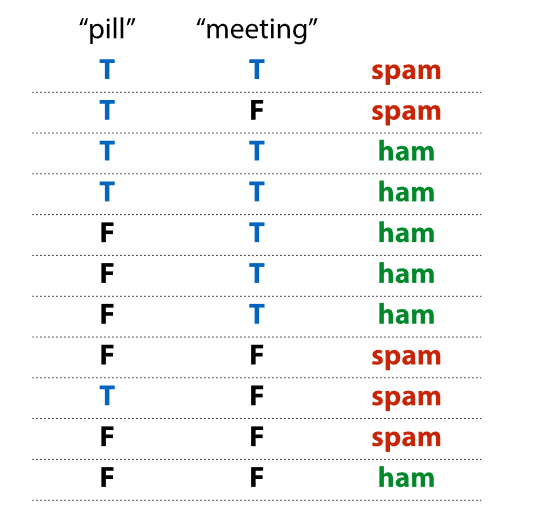
\includegraphics[width=0.3\textwidth]{assets/spamclassifier.png}
\end{figure}

We want to built a generative classifier, so one which aims to learn the distribution of a feature space given the class. By naive bayes we can do this for each feature independently and just multiply the probabilities.\\
For our example, assuming $X_1 = \text{pill}$ and $X_2 = \text{money}$ we express the probabilities as: 
\begin{align*}
    p(X_1 = T\mid \text{ham}) & = \frac{2}{6} \\
    p(X_1 = F\mid \text{ham}) & = \frac{4}{6} \\
    p(x_2 = T\mid \text{spam}) & = \frac{3}{5} \\
    p(x_2 = F\mid \text{spam}) & = \frac{2}{5} \\
\end{align*}

Now we can use these probabilities to calculate the probability of a new email being spam or not, for example say we had a new email with the features `pill' and `meeting'. \\
The probability of it being ham is proportional to the probability of seeing a ham email with the observed features and the probability of it being a ham email to begin with. Formally we can express this as:
\begin{align*}
    p(\text{ham}\mid X_1=T, X_2=T) & \propto p(X_1=T, X_2=T\mid \text{ham})p(\text{ham}) \\
    & = p(X_1=T\mid \text{ham})p(X_2=T\mid \text{ham})p(\text{ham}) \\
    & = \frac{2}{6}\times\frac{5}{6}\times\frac{6}{11} \\
\end{align*}

\subsubsection*{Laplace smoothing}

Naive bayes can run into issues with for some features a particular value does not occur thus giving a probability of 0. Its a problem because it causes the entire naive bayes probability to be 0. We can solve this by using smoothing.

\begin{definition}[pseudo-observations]
    Pseudo-observations are a type of smoothing where for each possible value, we add one instance where all features have that value. In a large dataset the impact of this is minimal and there exist further techniques to minimize the impact even more.
\end{definition}

We can use $\lambda$-smoothing to further minimize the impact of the pseudo-observations by reducing their weight among the other observations. Comparing unsmoothed, smoothed, and $\lambda$-smoothed using our spam classification we get the following expressions.

\begin{figure}
    \centering
    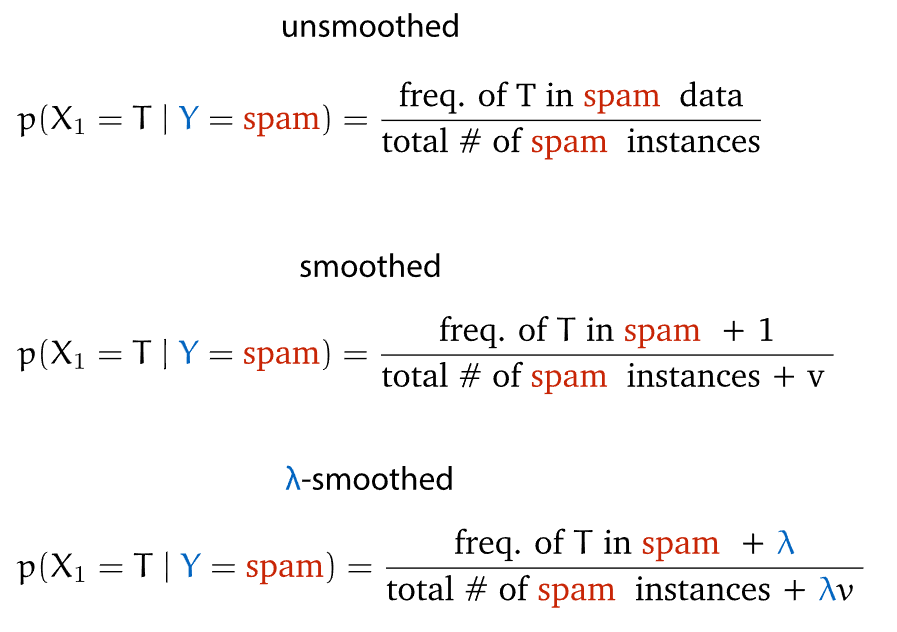
\includegraphics[width=0.5\textwidth]{assets/smootheddata.png}    
\end{figure}

\section{Logistic regression}

\begin{definition}[Logistic regression]
    Logistic regression is a type of \textit{discriminative} classifier that learns to map features directly to class probabilities without using bayes rule.
\end{definition}

\subsection{Logistic sigmoid function}

The logistic sigmoid function is a function that maps any real number to the range $[0, 1]$. It is defined as:
\[
    \sigma(x) = \frac{1}{1+e^{-x}} = \frac{e^x}{1+e^x}
\]
Some important properties of this function are: 
\begin{itemize}[leftmargin=*, noitemsep]
    \item symmetry: $\sigma(-x) = 1 - \sigma(x)$
    \item derivative: $\sigma'(x) = \sigma(x)(1-\sigma(x))$
\end{itemize}

Both of these are properties which make analysis easier.

\subsection{Logistic regression model}

In a basic logistic regression model we seem to try and treat a binary classification problem as a regression problem. All classes are assigned probabilities (e.g. probability of being positive) which constraints them to the range $[0, 1]$. \\
The decision boundary also has to be constrainted into this range which is where the logistic sigmoid function comes in. Given a hyperplane $\mathbf w ^\intercal \mathbf x + b$ we constrain it using the sigmoid function  s follows: 
\[
    c(x) = \sigma(\mathbf w ^\intercal \mathbf x + b)  
\]
From this for a good choice of $\mathbf w$ and $b$ we will get a probability distribution that assigns high probabilities to positive instances and low probabilities to negative instances. To see how well our model is we need a loss function.

\subsection{Logarthmic loss}

\begin{definition}[Logarithmic loss]
    Logarithmic loss (log loss/(binary) cross-entropy loss) is a loss function based on the maximum likelihood estimator.  
\end{definition}

Similar to the maximum likelihood estimator we some data $\mathbf x$, our two parameters $\bvec w$ and $b$. Where we are looking for a combination that maximumizes the probability of seeing the data we saw. We can call the probability distribution the classifier produces for $\bvec x$ , $q_\bvec x$. So the probability of a class $C$ conditioned on the data $\bvec x$ is given by:
\[
    q_\bvec x(C) = p(C\mid \bvec x)  
\]
In the case of binary classification for a positive and negative class we have for example 
\[
    q_\bvec x(\text{Pos}) = 0.1 \quad q_\bvec x(\text{Neg}) = 0.9  
\]

We can then express the probability of seeing our data $D$ as a function of the probability distribution $q_\bvec x$ as follows:
\[
    p(D) = \prod_{x, C\in D} q_x(C)  
\]
Since we assume the instances in our data are independent the probabilities of all class labels are just the product of the probabilities of the individual class labels given the data. Now to create an equation for the log loss. Firstly the main idea here is that we want to maximize the log-probability of the class labels given the data. We can express this as: 
\[
    \argmax_q \prod_{C, \bvec x} q_\bvec x (C) = \argmax_q \log \prod_{C, \bvec x} q_\bvec x (C)  
\]
Since we generally want to minimize the loss we multiply the above expression by $-1$ to get the following: 
\[
    \argmax_q \log \prod_{C, \bvec x} q_\bvec x (C) = \argmin_q -\log \prod_{C, \bvec x} q_\bvec x (C) 
\]
We can then move out the multiplication of the logarithm to turn the expression into a sum 
\[
    \argmin_q \sum_{C, \bvec x} -\log q_\bvec x (C)
\]
Finally we separate the data into positive and negative instances and express the loss as:
\[
    \argmin_q \sum_{x\in \bvec x _\text{Pos}} -\log q_x (\text{Pos}) - \sum_{x\in\bvec x_\text{Neg}} -\log q_x (\text{Neg})  
\]

This loss function says that 
\begin{itemize}[leftmargin=*, noitemsep]
    \item For the positive points we want to maximize the log-probability of being positive
    \item For the negative points we want to maximize the log-probability of being negative 
\end{itemize}
\newpage
In practice the log loss tries to maximize the sum of the logarithms (minimize the negative logarithm).

\begin{figure}[!h]
    \centering
    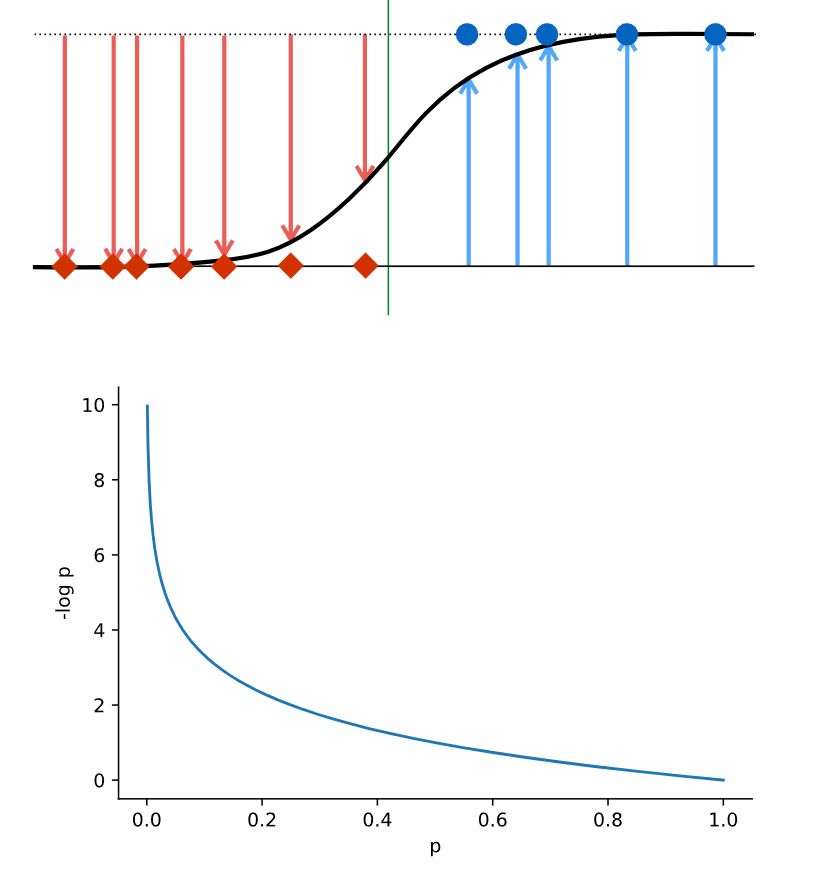
\includegraphics[width=0.4\textwidth]{assets/logloss.png}
\end{figure}

In the bottom we see the effect of taking the negative logarithm: 
\begin{itemize}[leftmargin=*, noitemsep]
    \item In the case of a low probability the loss is quite high 
    \item In the case of a high probability, so where the rod in the upper diagram is close to the instance, the corresponding loss is low. 
\end{itemize}
Intuitively this means that for the loss function low probabilities are penalized more than high probabilities, analagously to how with least squares we penalize large errors more than small errors by squaring the residuals between the predicted and actual values.

\subsubsection*{Minimizing loss}

To minimize loss for logistic regression we use \textit{gradient descent} on the loss function. As a quick recap this is our loss function: 
\[
    \text{loss}(\bvec w, b) = -\sum_{x\in \bvec x _\text{Pos}} \log q_x(P) - \sum_{x\in\bvec x_\text{Neg}} \log (q_x(N))
\]

First we can apply the sum rule to yield the following 
\begin{align*}
    \frac{\partial \text{loss}(\bvec w, b)}{\partial w_i} & = \sum_{x\in \bvec x _\text{Pos}} -\frac{\partial}{\partial w_i} \log q_x(P) + \sum_{x\in\bvec x_\text{Neg}} -\frac{\partial}{\partial w_i} \log q_x(N) \\
\end{align*}

First we can look at the positive term. To simplify the derivation we assume $y = \bvec w ^\intercal \bvec x + b$. 
\begin{align*}
    -\frac{\partial}{\partial w_i}\log q_x(P) & = -\frac{\partial}{\partial w_i}\log \sigma(y) \\
    & = -\frac{\partial \log \sigma(y)}{\partial \sigma(y)} \times \frac{\partial \sigma(y)}{\partial y} \times \frac{\partial y}{\partial w_i} \quad (\text{chain rule 2x}) \\
    & = -\frac{1}{\sigma(y)} \times \sigma(y)(1-\sigma(y)) \times x_i \quad (\text{basic derivatives}) \\
    & = -(1-\sigma(y))x_i = -q_x(N)x_i \quad (\text{simplification and rewriting})
\end{align*}

In the context of graident descent this value is the one we want to subtract from the current $w_i$ to better fit the classifier to the particular point $x$. \\ \\ 
As an example we can assume the clasifier does badly, so to a positive point $x$ it assigns a large prob. for the negative class, that is $q_x(N)$ is large. If $x_i$ is a large positive value, then gradient descent will subtract a large negative number $-q_x(N)x_i$ from $w_i$. This increases the sum $\bvec w ^\intercal \bvec x$ and thus the probability of the positive class. The same logic applies in the converse case.\\ \\ 
If a classifier does well then $q_x(N)$ is close to 0, and this particular instance has little influence on the gradient descent step. \\ \\
Deriving the second term we get the same form but with $q_x(P)$ instead of $q_x(N)$ and a minus. This gives us the partial derivative of the loss function with respect to the weights.
\[
    \frac{\partial}{\partial w_i} \text{loss}(\bvec w, b) = -\sum_{x\in \bvec x _\text{Pos}} q_x(N)x_i + \sum_{x\in\bvec x_\text{Neg}} q_x(P)x_i
\]

\subsection{Logistic regression application summary}

The summary of how to apply logistc regression is as follows: 
\begin{enumerate}[leftmargin=*, noitemsep]
    \item Use the sigmoid function to turn a linear classifier into a discriminative probalistic classifier
    \item Use log loss, so the maximize the log-likelihood of the data given the model
    \item Derive the gradient of the loss function and use gradient descent to minimize the loss, that is, search for good weights 
\end{enumerate}

One thing of note regarding the desicion boundary is that its still a hyperplane in the 2D case. We just changed the loss function by using it to fit the curved sigmoid function through the probability values in the data. So its kind of like regression but the actual hyperplane $w^\intercal x + b$ is what ends up being the decision boundary.

\subsection{Logistic regression overall summary}

\begin{itemize}[leftmargin=*, noitemsep]
    \item Use the logistc sigmoid to provide class probabilities from a linear classifier.
    \item Use $-\log p(\text{class}\mid\text{features})$ as a loss function.
    \item Points near the decision boundary get more influence that points away
    \item Log loss generalises naturally to multi-class classification
\end{itemize}

\section{Information theory}

\subsection{Probabilities and codes}

We can simulate things like a 6 sided die via a coinflip. We do this by using different combinations of coinflips to represent the different sides of a die. This in turn then also associates each encoded die roll with a corresponding probability depending on the combination of coinflips. 
\newpage
If we represent these combinations in conjunction with including reset branches we can represent any probability distribution using this encoding method.
\begin{figure}[!h]
    \centering
    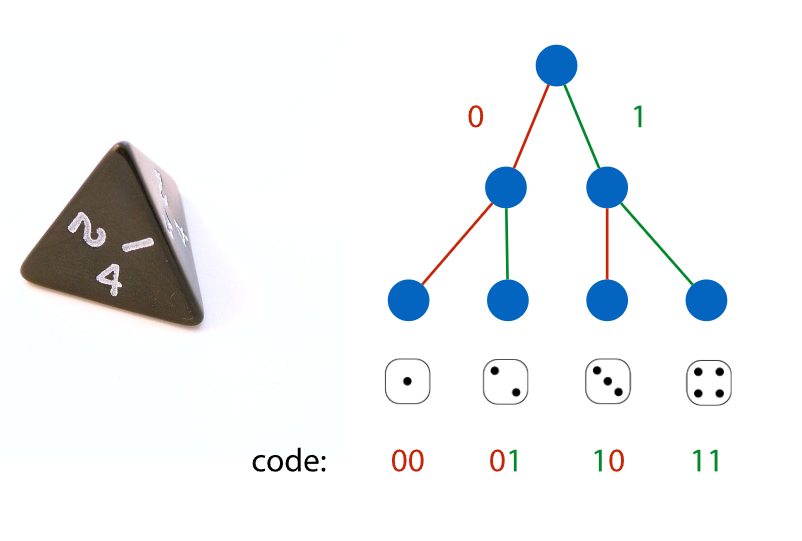
\includegraphics[width=0.4\textwidth]{assets/prefixfreecode.png}
\end{figure}
\begin{definition}[Prefix-free tree]
    A prefix-free tree is a tree which encodes some probability distribution. The resulting codes are prefix-free due to the fact that no code word will be a prefix of any other code word, which comes with the implication that given a prefix-free tree no delimiters are needed to separate the code words.
\end{definition}

There is a relation between the length of a code we assign its outcome and its probability. For example the more coinflips we require to get to a particular outcome, the lower the probability that we will get there, and the longer the code.\\  \\ 
\subsection{Codelengths}

If we define $L(x)$ as the length of the code for outcome $x$ we can first see that we need to for example flip a coin 3 times to get to a codeword of length 3, generalizing this: 
\begin{align*}
    p(x) & = \frac{1}{2}\times\cdots\times\frac{1}{2} \\ 
    & = \left(\frac{1}{2}\right)^{L(x)} \\
    & = 2^{-L(x)} \\ 
    \implies L(x)  & = -\log p(x)
\end{align*}

The key takeaway here is that the negative logarithm of the probability of an outcome is the length of the code for that outcome. \\ \\ 
For any distribution $L$ we can find a prefix-free code so that the value $-\log p(x)$ and the code-length $L(x)$ differ by no more than 1 bit for any outcome $x$. Formally this is expressed as 
\[
    \mid -\log_2 p(x) - L(x) \mid \leq 1  
\]
\subsection{entropy}

\begin{definition}[Entropy]
    Entropy is the measure of the expected number of bits we will have to use per outcome. Its the codelength of each outcome multiplied by its probability, summed over all outcomes. Formally, if we encode $X$ with the corresponding code $p$, our expected codelength is given by: 
    \begin{align*}
        H(p) & = E_p [L(x)] \\
        & = \sum_{x\in X} p(x)L(x) \\
        & = -\sum_{x\in X} p(x)\log p(x) \\
    \end{align*}
\end{definition}

\subsubsection*{Uncertainty}

Entropy is a measure of uncertainty about the outcome of a distribution. In other words it measures how uniformly spread out the probability mass is among the outcomes.

\begin{figure}[!h]
    \centering
    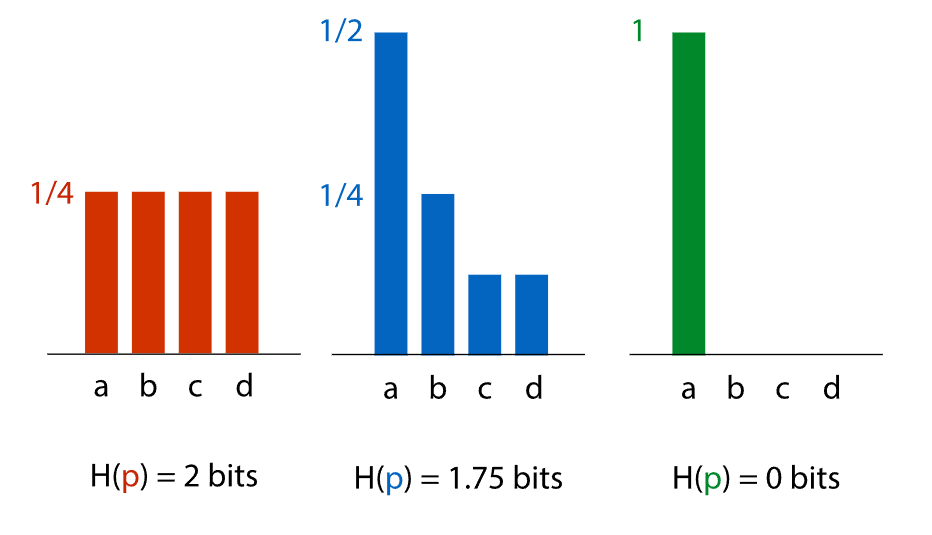
\includegraphics[width=0.6\textwidth]{assets/entropy.png}
\end{figure}

\subsection{Cross-entropy}

\begin{definition}[Cross-entropy]
    Cross-entropy is the expected codelength if we use $q$, but then the data comes from $p(x)$. So instead of using a code that corresponds to our data $p$ to encode it we use some other code based on a distribution $q(x)$. Formally this is expressed as:
    \begin{align*}
        H(p, q) & = E_p[L_q(x)] \\
        & = -\sum_{x\in X} p(x)\log q(x) \\        
    \end{align*}
\end{definition}

Some notes regarding cross-entropy:
\begin{itemize}[leftmargin=*, noitemsep]
    \item The code corresponding to $p$ provides the best expected codelength out of all possible prefix-free codes.
    \item The cross-entropy is a good way to quantify the distance between two distributions.
\end{itemize}

\subsubsection*{Kulback-Leibler divergence}

\begin{definition}[KL divergence]
    This is a function which is a measure of how far apart two distributions are. It's not symmetric and is defined as the difference between the cross-entropy and the entropy. Formally this is expressed as:
    \begin{align*}
        KL(p, q) & = H(p, q) - H(p) \\
        & = -\sum_{x\in X} p(x)\log \frac{q(x)}{p(x)}
    \end{align*}
\end{definition}

\subsection{Generalizing to continous and discrete space}

We can create a general expression for entropy and KL divergence using the expected operator which implies we integrate for continous spaces and sum for discrete spaces. Formally this is expressed as:
\begin{align*}
    H(p) & = -\int p(x)\log p(x)dx = -E_p[\log p(x)] \\
    KL(p, q) & = -\int p(x)\log \frac{q(x)}{p(x)}dx = -E_p[\log \frac{q(x)}{p(x)}]
\end{align*}

\subsection{Log loss as cross-entropy loss}

We can rewrite the log-loss function using the function for cross entropy loss as follows 
\begin{align*}
    \text{loss}(q) & = \sum_{x\in X}H(p_x, q_x) \\ 
    & = \sum_{x\in X} p_x(P)\log q_x(P) + p_x(N)\log q_x(N) \\
    & = -\sum_{x\in X} \log q_x(P) - \sum_{x\in X}\log q_x(N) \\
\end{align*}

Some interpretations we can make about this relation: 
\begin{itemize}[leftmargin=*, noitemsep]
    \item If we minimize $-q_x(P)$ in logistic regression, we are also minizing the amount of bits we would need to transmit to comunicate that $x$ is of the positive class.
\end{itemize}

\subsection{Minimum Description Length principle (MDL)}

Compression is similar to learning: 
\begin{enumerate}[leftmargin=*, noitemsep]
    \item Look at some data 
    \item Try to isolate recorruding patterns in the data, using coding and entropy
\end{enumerate}

\subsubsection*{Sender and receiver framework}

The SR framework can be described as follows: 
\begin{enumerate}[leftmargin=*, noitemsep]
    \item Sender sees some data 
    \item Sender and receiver can come up with any scheme to commmunicate the data 
    \item Data has to be sent using the scheme 
    \item Data must be perfectly reconstructed/decoded by the receiver
\end{enumerate}

\subsubsection*{Two part coding}

The two part coding scheme can be described as follows:
\begin{enumerate}[leftmargin=*, noitemsep]
    \item Tje semder amd receiver agree beforehand on a family of models (e.g. normal distribution, indexed by parameters $\mu$ and $\sigma$)
    \item Once the sender has seen the data, they send the model best suited for the data (e.g. by sending the parameters $\mu$ and $\sigma$ for the chosen model)
    \item The sender uses the model to encode the data and sends it over 
    \item The receiver uses the model to decode the data
\end{enumerate}

The best choice of model is the one that minimizes the cost of communication the model and the data given the model.

\end{document}